\documentclass[12pt]{article} 
\usepackage{amsmath} 
\usepackage[dvips]{graphicx}
\usepackage{multirow} 
\usepackage{geometry} 
\usepackage{pdflscape}
\usepackage[labelfont=bf]{caption} 
\usepackage{setspace}
\usepackage[running]{lineno} 
% \usepackage[numbers,sort]{natbib}
\usepackage[round]{natbib} 
\usepackage{array}
\usepackage[table]{xcolor}

\newcommand{\methods}{\textit{Materials \& Methods}}
\newcommand{\SI}{\textit{Appendix}~}

\topmargin -1.5cm % 0.0cm 
\oddsidemargin 0.0cm % 0.2cm 
\textwidth 6.5in
\textheight 9.0in % 21cm
\footskip 1.0cm % 1.0cm

\usepackage{authblk}

\title{Participation in stable motifs delays extinction in simulated food webs}

% - in intro/discussion, make it clear that this is adding a new layer of meaning to differences/changes in species roles rather than trying to put motifs as the best way to predict extinctions.

% 1st Theo Bio, then PeerJ. 
% Reviewers: Jon Borrelli, Benno Simmons, Daniel Stouffer, Tim Poisot, Eva Delmas
% To SI: PCA axes, extinction order correlations
% Main text: permanova shows that roles are important, participation to identify which motifs are most strongly assoc. with stability.
% Kate to work on coverletter, language edits
% Need abstract, ?graphical abstract?, author contributions,  
% Need 3-5 bullet point highlights, submitted as a separate file. 
% No obvious word limits?

\author{Alyssa R. Cirtwill$^{1\dagger}$, Kate Wootton $^{2}$} 
\date{\small$^1$Department of Ecology, Evolution, and Plant Sciences\\ 
Stockholm University\\
Stockholm, Sweden\\
\medskip
\small$^2$ Swedish Agricultural University\\
Uppsala, Sweden\\
\medskip
$^\dagger$ Corresponding author:\\
alyssa.cirtwill@gmail.com\\
 }

\renewcommand\Authands{ and }

\begin{document} 
\maketitle 
\raggedright
\setlength{\parindent}{15pt} 


\section{Keywords}

	species roles; disturbance; competition; three-species chain; omnivory


\section{Abstract}


\section{Introduction}

	The connections between food-web structure and the extinction risk of species within a web have interested ecologists since at least the 1970's~\citep{May1972}. After early findings suggested that a large, randomly-connected network is unlikely to retain all species after small perturbations~\citep{Gardner1970,May1972}, non-random structures that might stabilize food webs were quickly identified. These structural features include nestedness~\citep{Allesina2012,Sauve2014}, modularity~\citep{Sauve2014,Thebault2010} and skewed distributions of link strengths~\citep{McCann1998,Gross2009,Rooney2012,Wootton2016}.
	
	
	Although important, these global-scale properties can mask important differences in  network structure~\citep{Simmons2019}, and do not provide information about differences between species within the same network~\citep{Cirtwill2018FoodWebs}. 
	Two networks with the same connectance and similar values of nestness and modularity may still have quite different meso-scale arrangements of links. 
	These meso-scale structures, described by frequencies of \emph{motifs} (unique patterns of $n$ interacting species), define the local neighbourhood of a focal species and reflect its direct and close indirect interactions (Fig.~\ref{motifs}).
	
	
    In addition to providing species-level information on network structure, there are early indications that some meso-scale structures may tend to stabilize food webs~\citep{Prill2005,Borrelli2015,Monteiro2016}. 
    This possibility is supported by the fact that empirical food webs tend to contain more \emph{three-species chains} and either more \emph{omnivory} (\emph{sensu}~\citealp[]{Thompson2007b}) motifs or more \emph{apparent competition} and \emph{direct competition} motifs than random networks~\citep{Stouffer2007}. 
    These four motifs make up, on average, about 95\% of all three-species motifs in food webs~\citep{Stouffer2010b}. 
    The high frequencies of these four motifs in oberserved networks suggest that they may be beneficial to the network containing them, or in other words, that more stable motifs appear more frequently in empirical food webs because unstable motifs are more likely to disappear as the species within them go extinct~\citep{Borrelli2015,Borrelli2015a}.

	When modelled in isolation, three species arranged in \emph{three-species chain}, \emph{apparent competition}, \emph{direct competition}, and \emph{omnivory} motifs are more likely to all persist than species arranged in other motifs~\citep{Borrelli2015a}.
	By damping perturbations and maintaining more constant populations of the species participating in them, these `stable' motifs may contribute to the stability of the network as a whole~\citep{Borrelli2015a}. 
    The greater chances of maintaining all species in a stable motif could explain the over-representation of these motifs in empirical food webs if species and interactions in less-stable motifs are more likely to be ``pruned'' from empirical communities over time. We expect that stable structures will endure for longer than unstable ones, and so it is not surprising that stable structures should be over-represented in empirical communities~\citep{Borrelli2015}.


    Testing this hypothesis is complicated by the fact that species' motif roles are not independent of other aspects of fine-scale network structure. 
    In particular, a species' degree (number of predators and prey) is likely to strongly affect its motifs role.
    The more interaction partners a species has, the more motifs in can participate in (Fig.~\ref{motifs}).
    This is likely to lead the species to participate in a wider variety of motifs as well as participate more frequently in the four common, stable motifs.
    Species with high in-degrees (more prey) are also generally less likely to go extinct, as are species at lower trophic levels~\citep{Cirtwill2018FoodWebs}.
    Any test for a relationship between motif roles and time to extinction should therefore take degree and trophic level into account.

   \begin{figure}[hb!]
        \centering
        % 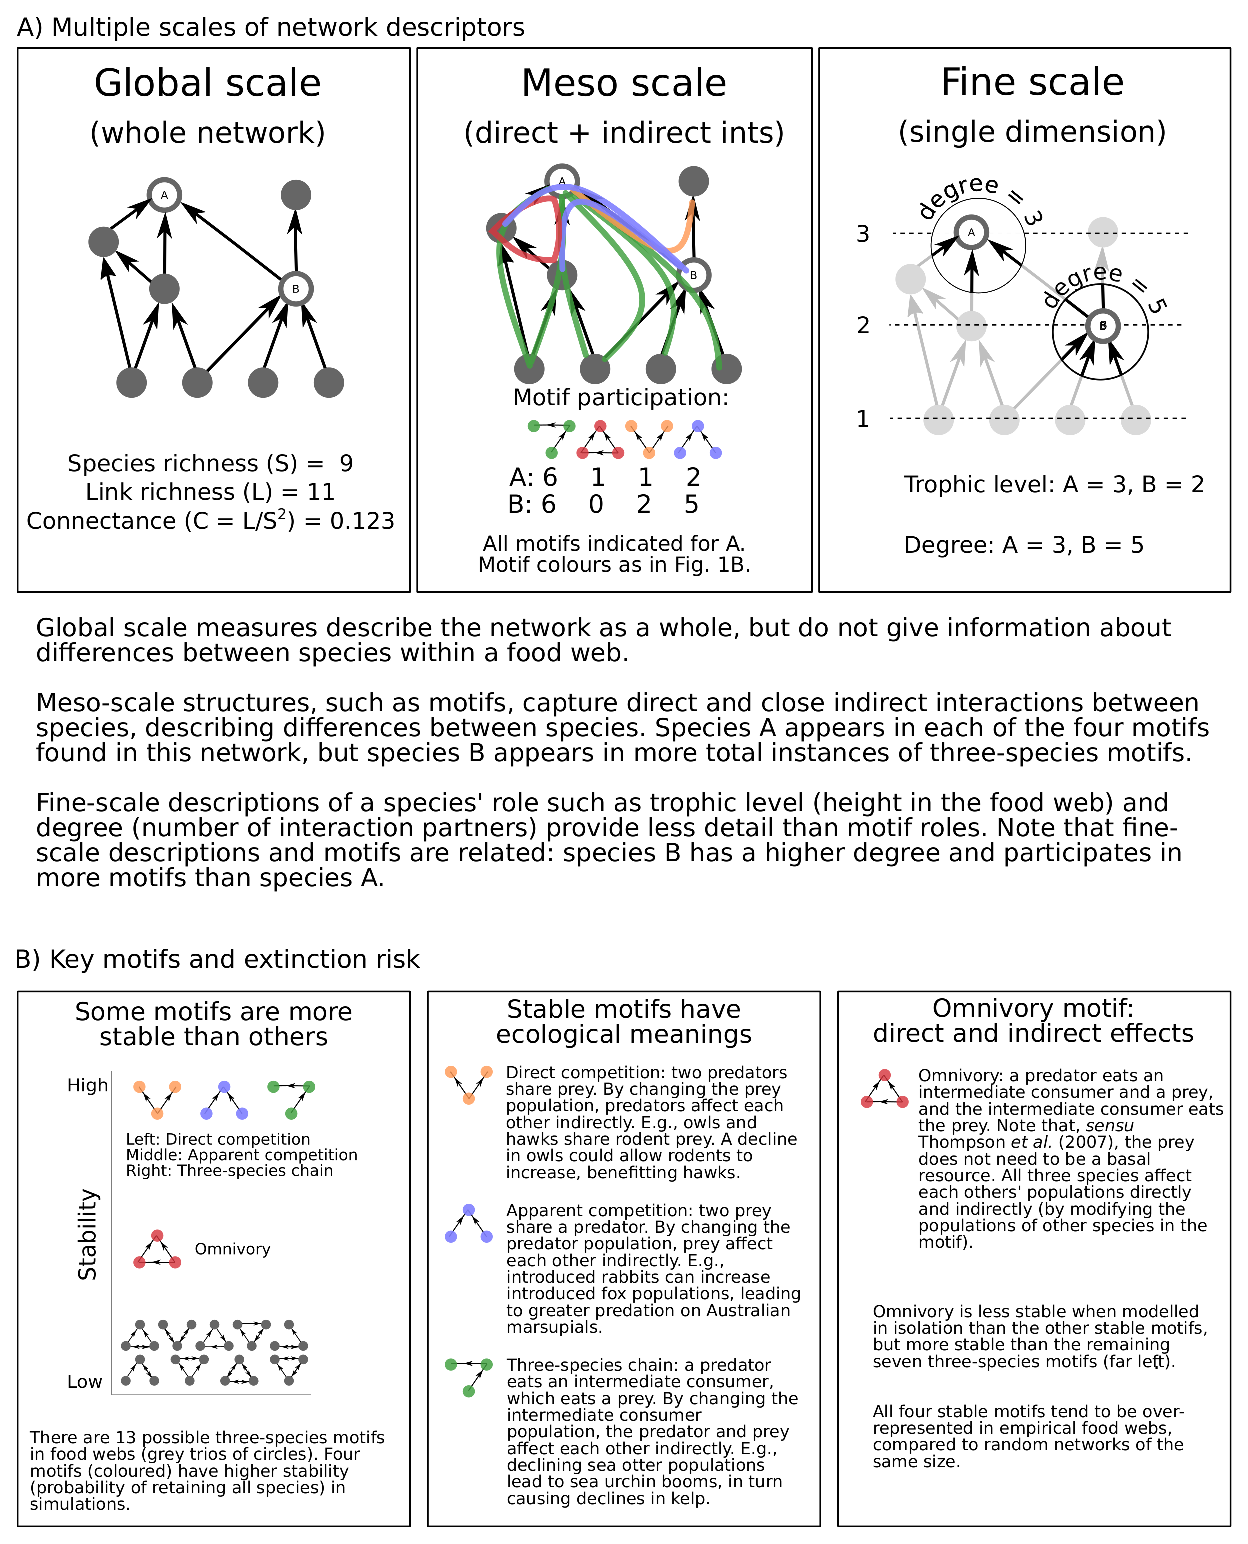
\includegraphics[width=\textwidth]{figures/motifs_box.eps}
        \caption{\small \textbf{A}) Food web structure can be described at several different scales. Global scale measures like species richness (S), link richness (L), and connectance (C = L/S$^2$) describe the network as a whole but do not give information on how the extinction risk differs for species within a food web (i.e., species A and B; labelled). Differences between these species can be described by their participation in three-species motifs: \emph{meso-scale} structures that capture direct and close indirect interactions between species. Here, a species' \emph{motif role} is a vector describing the number of times it appears in each motif. Only four motifs are included in the toy network shown, indicated by small diagrams to the right. Finer-scale descriptions of a species' role such as trophic level (TL; height in the food web) and degree (number of interaction partners) also capture differences between species but do not provide as much detail as motif roles.\\
        \textbf{B}) There are 13 unique three-species motifs. Four of these (highlighted with coloured backgrounds and shown in colour in the inset network) are of particular interest. These four motifs have been identified as more stable than other configurations of interacting species and as likely to stabilize the food web as a whole. Moreover, these motifs have clear ecological meanings and have been studied in isolation as well as in food-web contexts.\\
        The direct competition motif (orange, top left) includes two predators which share a common prey. The predators are expected to affect each other by modulating the prey's population even if they do not physically encounter each other. Similarly, the apparent competition motif (blue, top middle) includes two prey which share a common predator and are expected to affect each other by modulating the predator's population. 
        The three-species chain (green, top right) includes a top, intermediate, and bottom species and the top and bottom species are expected to affect each other through effects on the intermediate species' population. The omnivory motif (\emph{sensu} Thompson \emph{et al.}, 2007) motif (red, middle) includes a top, intermediate, and bottom species where both the top and intermediate species consume the bottom species. Note that the bottom species does not necessarily need to be a basal resource. This motif includes both direct and indirect effects between all pairs of species.}
        \label{motifs}
    \end{figure}


	Given these early indications that some motifs are more stable than others, we may also expect that a species' role-- here defined as the frequency with which it participates in different motifs --could affect its probability of extinction following a perturbation. Specifically, we expect that species participating more frequently in the stable motifs identified by~\citet{Borrelli2015a} are less likely to go extinct than species whose roles are dominated by other motifs. Here, we investigate this question by simulating the removal of species from simulated networks at stable equilibria. We test 1) whether species' roles are related to their time to extinction following the removal of another species in the network, 2) whether participation in particular motifs (especially the stable motifs described above) is correlated with time to extinction, and 3) whether these correlations are driven by potential relationships between species' participation in various motifs and simpler definitions of species roles (degree, trophic level). Our overall aim is to establish whether changes in species' roles can, in future, be used to evaluate whether species are at increasing or decreasing risk of extinction.


	% Approx. 1000 words of introduction

	% Stability of biological networks has been related to the frequency of different motifs.
	% - Prill2005 transcription networks are more stable if they contain more "structurally stable" motifs (motifs whose structures mean a larger parameter space of signs and strengths is stable) motifs. Most stable motifs were apparent competition, direct competition, chain, omnivory (all fully structurally stable - will return to steady state if perturbed without oscillations), then quite a sharp drop before other motifs inc. two-way motifs and one-way loop. Two-way loop was least stable. Stable motifs are more abundant in biological networks. Three classes: I) acyclic graphs (no two-way links), fully stable; II) graphs with one two-way link; III) more complicated circuits (two-way link plus a loop, two two-way links, one-way loop, etc).
	% - Stouffer2007 showed chain, omnivory over-represented but both competitions under-represented compared to random in 10/16 empirical webs, competition over-represented and omnivory under in 6/16. Double-loop also over-represented... important to distinguish between abundance and statistical over-abundance of motifs. Motifs in empirical networks consistent with the niche model and not nested-hierarchy. 
	% - Stouffer2010 only relevant for pointer to Stouffer2007
	% - Stouffer2010b average 95\% of all motifs are chain, omnivory, apparent and direct competition. In isolation, species in tri-trophic chain most likely to all persist, then omnivory, then apparent competition, the direct competition. More species persist in food webs with many chains and omivory, persistence decreases with more apparent and direct competition.
	% - Stouffer2005 empirical connectance ranges 0.026-0.315 (25 to 155 trophic species)
	% - Stouffer2012 54 distinct roles across 32 webs, up to 22 roles per web (not related to size of web or taxonomic diversity). 46 roles for intermediate species, remainder are basal/int and int/top. Closely related species have similar roles, species with similar roles have similar benefits to their community (based on how much stability increases/decreases when a single motif is added). *Check SI for more details on benefit analysis.
	% - Kondoh2008 Intraguild predation modules can be stable if 1) prey is a superior competitor for the resource or 2) extra-module forces such as additional resources exist that benefit the prey more than the predator. In Caribbean food web, all but two species participate in at least 1 IGP module and three sharks are in \>1000. Intrinsically-stable modules were over-represented. Non-intrinsically stable modules were more likely to have external influences favouring prey. If externally-stablised IGP are stabilised by other IGP, may be vulnerable to perturbations. Expect more external stabilisation from internally-stable IGP. This is exactly what was found.
	% - Borrelli2015 Systems may be nonadaptively selected for stability by preferential removal of nonstable systems (e.g., culling interactions that lead to oscillations giving low abundances, )
	% - Rip2010 Modules that weaken interactions should stabilize the network, looking at "biparallel motif" as one such option - two chains linked at top and bottom. Tested empirically in microcosms, isolated. Generalist consumer de-synchronised its resources, stabilizing community. 
	% - Klaise2017 Disagree that the generalized niche model produces networks with similar motif profiles. Clustered food webs with similar profiles using a "hierarchical, agglomerative clustering algorithm based on the Pearson’s correlation coefficient (r)". Distance between webs is sqrt(2*(1-r)). Distances clustered using UPGMA (average linkage) algorithm. Trophic coherence (propensity of species to consume exclusively at the TL below themselves) tunes motif frequencies between two "families", only one of which is generated by the niche model. Main difference is whether omnivory is strongly over- or under-represented.
	% - Baiser2015 Local networks resemble regional ones if all trophic groups are sub-sampled with similar frequencies. Not particularly relevant.
	% - Monteiro2016  [Haydon1994, May1972, Sterner1997] show that modules are more stable with fewer interactions, small variance in interaction strengths, self-damping processes. Used Jacobian to identify stability of each 3- and 4-species motif, looked at frequencies in empirical networks. AC, DC, chain, and omnivory were all stable (omnivory could also be unstable). More stable motifs appeared more frequen tly. Same for 4-species motifs (4\% were stable). Omnivory ranging stable-unstable can explain contradictory results for omnivory in other studies.
	% - Gross2009 High variability in interaction strengths stabilizes small webs, destabilizes large ones. Stability also enhanced by generalist predators (high TL) and very vulnerable intermediate consumers. Used very large suite of simulated networks. No talk of motifs.
	% - Dambrot 2017 Having few loops seems to stabilize networks, but we don't know how they come to be un-loopy. Probably trophic coherence again. Not super relevant.
	% - Otto2007 Bioenergetic model to explore body-mass ratios and stability of tri-trophic chains. Only particular ratios are stable. Body mass also correlates with degree (+ with number of prey, - with number of predators)
	% - Bascompte2005 Ealier work (McCann1998) emphasizes stabilizing role of omnivory but nobody tested whether omnivory over-represented. Apparent competition and intraguild predation (4-sp, two chains with one middle sp. eating the other) more common than expected, omnivory more variable. 
	% - Rooney2012 Existence of fast and slow energy channels is stabilizing because it de-synchronises prey populations. Interactions in slow channels also tend to be weaker. Mostly about size and stability.
	% - Smith2015 Technical argument about how to standardize community matrices for calculating eigenvalues. Boring (sorry Gyuri)
	% - Allesina2008 Pred-prey networks are more likely to be stable than random ones. Varied off-diagonal C from 0.05 to 0.5 with steps of 0.025, size from 10 to 100 with steps of 5. 1000 webs of each size. Determined stability based on percentage of eigenvalues with negative real parts. Did not allow two-way links. Predator-prey networks are more stable than those where signs of interactions are random. Still stable if +/+ and -/- interactions present but less common than pred/prey. Weak interactions not necessary. Short cycles (self-regulation, predator-prey "cycles") may be key, will have greater influence bc. they are smaller. They believe they're supporting the "stable motifs lead to stable networks" lit.
	% - Borrelli2014 Food chains are generally 2-4 levels long. When weighted, usually 3 (Ulanowicz2013). Probably not because of inefficient transfer (productivity not strongly correlated with maxTL). Longer food chains take longer to stabilize following a perturbation. Looking at stability of mini-webs and larger random & niche model ones. Found that quasi sign-stability (a la Allesina2008) decreases with increasing chain length, dropping sharply after 3 for mini-webs to almost 0 for length 6.  
	% - Borrelli2015 This is the one about motifs and stability. Using Jacobian eigenvalue stability (return to equilibrium following small perturbation). Looked at sign stability of each motif in isolation, Z-scores in empirical webs. Chains, apparent competition, and direct competition were all more likely to be stable and over-represented. Omnivory was moderately likely to be stable, typically under-represented. Could indicate that unstable motifs are more likely to be "pruned", selecting for stability of the whole system. 
	% - German thesis Restricted to pairwise interactions and chains.
	% - Wootton2016a Pulse vs. press disturbance important. Used press disturbance because many anthropogenic effects thus, many affect one species disproportionately. Affected species may or may not be the one that goes extinct. Tested how web size and connectance affected resistance (size of disturbance required to cause extinction), how traits of disturbed species affected outcome. Found that smaller, less-connected networks were more resistant, focal extinctions more likely. 59\% of extinctions focal, 24\% of extinctions involve indirect interaction partners, 16\% of extinctions predators of focal species, 1\% of extinctions prey of focal species. Higher degree species were more llikely to cause extinction of predators, prey extinctions came from high S, high C webs with focal species with high degree. 


\section{Methods}

	\subsection*{Generating food webs}

		We simulated a suite of food webs based on the probabilistic niche model, which assigns predator-prey links based on the body-mass ratios between species~\citep{Williams2000,Delmas2017}. The meso-scale structure of such networks closely mimics that of empirical food webs~\citep{Stouffer2007}. To parameterize the model, we specified a predator-prey body-mass ratio of 3.065 based on the estimate for vertebrates (averaged across ecosystem and metabolic types) in~\citet{Brose2006}. We excluded reported body-mass ratios for invertebrates as these could include parasites and parasitoids, which are generally smaller than their prey, and because interactions among vertebrates are better represented in the food-web literature than interactions involving invertebrates. To ensure that we captured a variety of realistic community sizes and structures, we generated networks ranging between 50 and 100 species (in steps of 10) with connectances between 0.02 and 0.2 (in steps of 0.02). The range of network sizes was chosen to reflect moderately well-sampled empirical webs while working within our computational limits, while the range of connectances was chosen to cover that observed in empirical food webs~\citep{}. We generated a total of 100 networks with each combination of parameters, for a total of 6000 networks. All networks were simulated using the function "nichemodel" within the Julia language package \emph{BioEnergeticFoodWebs}~\citep{bioenergeticfw,Delmas2017}. If a simulated network contained any disconnected species (species without predators or prey) or disconnected components (a group of species connected amongst themselves but not to the rest of the network), the network was rejected and a new network simulated. Finally, networks where the path lengths between each species and a basal resource could not be resolved were rejected and new networks simulated.


		After assigning biomasses, we simulated community dynamics in order to obtain an equilibrium community. To ensure that species did not `recover' from unrealistically low biomasses, we considered a species extinct if it dropped below a threshold biomass of 1$\times10^{-5}$ and rejected the network. Community dynamics are based on Lotka-Volterra predator-prey models including density dependence and with type II functional responses for all species (please see~\citet{Delmas2017} for full details; all non-basal species were designated as vertebrates to ensure a good match between metabolic and predator-prey bodymass ratio values). Consumers were assumed to have no preferences such that the consumption rate $w_{ij}$ of $i$ eating $j$ is equal to $\frac{1}{n}$, where $n$ is the number of prey for predator $i$. If the network did not reach an equilibrium with all species persisting after 1000 time steps, a new set of initial population biomasses was applied and the simulation repeated until an equilibrium with all species persisting was obtained. 


	\subsection*{Calculating motifs and species roles}


		We were interested in whether species' roles at equilibrium are related to their response to a perturbation, in this case the removal of another species in the network. We defined each species' role as the number of times it appears in each unique three-species motif, following~\citet{Stouffer2012,Cirtwill2015}. As our focus is on how different motifs might affect extinction risk, we do not consider the different positions species may take within a motif. We expect that appearing more frequently in stable motifs (three-species chain, apparent and direct competition, and omnivory) will correlate with lower extinction risk while appearing more frequently in unstable motifs (those containing two- or three-species loops) will be related to higher extinction risk.	Note that cannibalistic links were ignored when calculating motif frequencies within a network and species' roles, although they were included when calculating connectance. As well as these 'raw' motif roles, we calculated 'degree normalized' motif roles for each species by dividing the number of appearances in each motif by the total number of times the species appears in any motif (as in~\citet{Cirtwill2015}). These 'normalized motifs' should control for differences in species' degrees (numbers of interaction partners). Finally, we also calculated 'network normalized' motif roles, defined as the z-score of the number of times a focal species appears in each motif compared to the number of times all species in the network appear in the focal motif.
		The degree normalisation allows us to test whether trends in stability with motif participation are due to differences in species' degrees, while the network normalisation allows us to test whether trends in stability with participation in different motifs are related to how unusual each species is within its community context.


		% Apart from motif-based measures of species' positions in their communities, we calculated their degrees and short-weighted trophic levels. Degree is simply the number of interaction partners for each species. A species' short-weighted trophic level is the mean of its shortest trophic level an prey-averaged trophic level. The shortest trophic level is calculated based on the length of the shortest food chain between the focal species and any basal resource. Basal resources are assigned a trophic level of one and other species are assigned a shortest trophic level of one plus the trophic level of their prey. Prey-averaged trophic level is calculated based on the set of all shortest food chains between the focal species and any basal resources. The focal species' prey-averaged trophic level is the mean trophic level of its prey plus one. These alternative topological measures will be used to evaluate how strongly species' motif roles are related to their response to perturbation compared to other measures of position within a network. These measures were used to test how consistent motif roles and motif participation are for species which share the same degree or trophic level. [[Need to add this formally once I do it.]]


	\subsection*{Perturbing networks}

		After identifying species' roles in the equilibrium networks, we perturbed the networks by removing a single species. After this removal, community dynamics were simulated for 50 rounds of 10 time-steps (500 time-steps total). After each round, any species with a biomass below our threshold of 1$\times10^{-5}$ was considered to have gone extinct and its biomass was set to 0. We recorded the biomass of each species after each round, as well as the round in which any additional extinctions occurred. After 500 time-steps, we reset the network to its original state (including all species). We then removed a new species and again simulated community dynamics. We repeated this process until all species had served as the initial removal.
		We then calculated the mean time to extinction across all removals as an overall measure of each species' vulnerability (\emph{Appendix SQ}, Supplemental Information). 
		Time to extinction was highly correlated across removals in all combinations of S and C, indicating that this is a robust measure.


	\subsection*{Testing effects of species' roles on time to extinction}

		\subsubsection*{Relating overall motif roles to time to extinction}

			To test for a relationship between persistence and species' overall roles, we therefore fit a series of PERMANOVAs relating dissimilarity in roles to differences in mean time to extinction.
			PERMANOVA is a multivariate analogue of classic ANOVA which, importantly, does not assume that response data are normally distributed~\citep{Anderson2001}.
			To avoid effects of network size and connectance on time to extinction, we fit separate PERMANOVAs for each combination of network size and connectance (60 PERMANOVAs in total).
			As conducting so many tests risks obtaining significant results by chance, we applied the correlated Bonferroni correction~\citep{Drezner2016} before evaluating significance.
			We calculated Bray-Curtis dissimilarity in the counts of each motif in the role of each species~\citep{Baker2015,Cirtwill2015} and related these dissimilarities to differences in mean time to extinction.
			We fit all PERMANVOAs using the R~\citep{R} function 'adonis' from the package \emph{vegan}~\citep{vegan} and calculated $p$-values using 9999 unstratified permutations.
            To support these PERMANOVAs, we fit a linear model testing whether the raw frequencies of each motif were related to mean time to extinction (\emph{Appendix SX}, Supplemental Information).


		\subsubsection*{Identifying the motifs most strongly related to time to extinction}

			While the PERMANOVA can tell us whether a species' role as a whole is related to its mean time to extinction, it does not reveal which motifs have the strongest effect on time to extinction.
			To answer this question, we used a partial least squares (PLS) regression to identify combinations of motifs which, together, explain substantial variation in time to extinction. 
			Similar to a principal components analysis (PCA), PLS involves projecting the observed variables (in this case, participation in different motifs) into a new space and identifying latent variables made up of linear combinations of the observed variables~\citep{Mevik2007}.
			In our case, these latent variables represent combinations of motifs which, together, explain substantial variation in persistence.
			As well as simply identifying key motifs, we were interested in understanding whether species achieve longer mean times to extinction because their roles contain greater proportions of certain motifs or because they participate in certain motifs more than other species within the same network.
			
			
			To distinguish between these two possibilities, we fit two separate PLS regressions.
			In the first, we used mean time to extinction as the response and network size, connectance, the interaction between size and connectance, in-degree (number of prey), shortest trophic level, and degree-normalized motif participation as predictors.
			We include network parameters and other measures of species degrees as these may affect the motif roles available to each focal species.
			In the second, we used the same variables except for network-normalized motif participation (i.e., $Z$-scores of participation).
			The first regression tests whether a species' absolute participation in different motifs affects its time to extinction (e.g., whether participating in more three-species chains leads to longer persistence).
			The second tests whether a species' participation in more or fewer of different motifs, relative to other species in the network, affects its time to extinction. 

			
			In order to test the predictive ability of both models, we initially fit them on the first 50 networks of each size and connectance combination, reserving the remaining 50 networks as test data.
			To prevent the non-motif predictors from exerting overly large influence on the models, we centred and scaled these predictors. 
			This ensured similar ranges between normalised motifs and the other predictors.
			We fit both regressions using the R~\citep{R} function 'plsr' from the package \emph{pls}~\citep{pls} and cross-validated the regressions using 10 randomly-selected segments of the data and re-fitting.
			This cross-validation allows us to select the optimum number of components to include in the regression.
			We selected the optimum model as the one with the fewest components with an mean squared error of prediction (MSEP) less than one standard deviation away from the best model.
			MSEP is a measure of the error obtained when re-fitting a PLS or PCA model on test data, and is commonly used to select the optimum number of components~\citep{Mevik2004})
			Model selection was performed using the R~\citep{R} function 'selectNcomp' from the package \emph{plsr}~\citep{pls} using the method 'onesigma'.
			After selecting the optimum number of components for each model, we re-fit the PLS regression including only the selected components. 
			We then summed the coefficients of each predictor across axes to obtain an overall measure of the effect of each predictor on mean time to extinction.


		\subsubsection*{Relating motif roles to other role definitions}
		
			Finally, we wanted to test the possibility that the relationships we observe between motif roles and time to extinction might be due to underlying relationships between species' numbers of interaction partners (degree) and their roles.
			Species with more interaction partners will participate in more motifs (as each combination of three interacting species represents a unique motif).
			These species might also participate in a more diverse set of motifs, or might have roles in which certain motifs are over-represented.
			To test these possibilities, we tested for relationships between a species degree and both the count and proportion of each motif in the species' role using a series of linear regressions (26 regressions total).
			All regressions included degree as a predictor and the count or proportion of the focal motif as a response and were fit with the R~\citep{R} base function 'lm'.
			Because species with no interaction partners (zero degree) would necessarily have no motif roles, we enforced an intercept of zero.
			As with our PERMANOVA analysis, fitting so many regressions runs the risk of obtaining significant results by chance.
			To increase the likelihood of detecting a true relationship between species' degrees and motif roles, we applied the correlated Bonferroni correction~\citep{Drezner2016} before evaluating significance of these regressions.


\section{Results}
	
    \subsection*{Relating overall motif roles to mean time to extinction}
    
		Species' roles were correlated with their mean time to extinction across all combinations of species richness and connectance (Table~\ref{permtable}). Taken individually, each PERMANOVA was significant (all $p$\textless0.025). Moreover, after applying the correlated Bonferroni correction~\citep{Drezner2016}, all PERMANOVAs remained significant. While values of the pseudo-$F$ statistic increased steadily with increasing species richness, $p$-values were similar across values of species richness and connectance (Fig.~\ref{permfig}). Neither the pseudo-$F$ nor the $p$-values demonstrate an obvious interaction between species richness and connectance.
        The frequencies of all motifs were significantly related to mean time to extinction, with motifs S1 and S4 having the largest positive associations with time to extinction after taking the observed numbers of each motif into account (\emph{Appendix SX}, Supplemental Information).


			\begin{figure}[hb!]
				\caption{Here we show (\textbf{A}) the pseudo-$F$ statistics and (\textbf{B}) the $p$-values for each PERMANOVA relating species' roles to their mean extinction order when all species in the web are separately removed. We fit one PERMANOVA per combination of species richness and connectance. $p$-values for each PERMANOVA are based on 9999 permutations, stratified by network. Symbols below the dotted line in \textbf{B} indicate a significant $p$-values.}
				\label{permfig}
				\includegraphics[height=.5\textheight]{figures/extinction_order/permanova_summary_paper_full.eps}
				\end{figure}




	\subsection*{Identifying the motifs most strongly related to mean time to extinction}

        After testing whether species' motif roles overall were related to mean times to extinction, we used PLS regressions to identify the motifs which were most strongly associated with persistence. 
        When using the raw (un-normalized) frequencies of motifs, the optimum model 
        
        
        To determine whether the key motifs differ when considering the shape of a species' role (i.e., degree normalization) or how a focal species compares to other in the same network (i.e., network normalization), we used partial least squares regressions with two different normalizations of species roles.
		When normalizing motif roles based on degree, the optimum model included 11 components.
		The first component explained 22.1\% of variation in mean time to extinction, with the remaining ten components explaining an additional 1\% or less.
		Taking the 11 components together, the proportion of a species' role made up by motifs D2 and S2 (Fig.~\ref{motifs}), trophic level, and the proportion of a species' role made up by motifs D4 and D1 all had large negative effects on mean time to extinction (i.e. species in these roles or with higher trophic levels went extinct faster) (Fig.~\ref{coefficient_sum}A).
		The proportion of a species' role made up by motifs S5, S1, and D2, as well as degree had substantial but smaller positive effects on mean time to extinction.


		When normalizing motif roles based on the network (i.e., defining motif participation as $Z$-scores), the optimum model included four components.
		Together, however, these four components explained only 14.8\% of variation in mean time to extinction (13.1\%, 1.0\%, 0.6\%, and 0.1\% respectively).
		Taking the four components together, trophic level had a large negative effect on mean time to extinction (Fig.~\ref{coefficient_sum}B).
		Connectance and over-representation of motif D4 had smaller negative effects on mean time to extinction, while over-representation of motifs S1, S4, S5, and D1 had smaller positive effects on mean time to extinction.


		\begin{figure}[hb!]
			\caption{Sum of loadings of normalized motif roles, degree, shortest trophic level (STL), web size (S), connectance (C), and their interaction (S:C) in the optimum number of axes in partial least squares regressions of mean time to extinction against all of the above predictors. We fit separate models for degree normalization (i.e., dividing counts of each motif by the total number of all motifs for the focal species) and network normalization (i.e., calculating $Z$-scores for each motif compared to all species in the network). Stable motifs are shaded in light blue.}
			\label{coefficient_sum}
			\includegraphics[height=0.5\textheight]{figures/PLS/total_coefficients.eps}
			\end{figure}


	\subsection*{Relating motif roles to degree}

		As expected, the count of all motifs increased significantly with increasing degree [[add a table if interesting]].
		The frequency of the four stable motifs (S1, S2, S4, and S5) increased most rapidly with increasing degree (Fig.~\ref{motif_vs_degree}A).
		Moreover, the proportion of a species' role which is made up by the four stable motifs also increased more rapidly with degree (Fig.~\ref{motif_vs_degree}B).
		The one-way loop motif and two-way motifs showed weak, although still significant, relationships with degree.


		\begin{figure}[hb!]
			\caption{As a species has more interaction partners, it participates in more motifs. \textbf{A)} The counts of the four stable motifs (S1, S2, S4, and S5) in a species' role increased most strongly with increasing degree. \textbf{B)} The proportion of a species' role made up by the four stable motifs also increased strongly with degree. In both panels, motifs are plotted in order of the strength of their relationship with degree and all relationships were significant. 95\% confidence intervals about the regression lines are too small to be visible in the current plot. In both panels, the four stable motifs are indicated by blue lines while unstable motifs are indicated by yellow lines.}
			\label{motif_vs_degree}
			\includegraphics[width=.75\textwidth]{figures/roles/motif_vs_degree.eps}
			\end{figure}


\section{Discussion}

	[[Subheadings just to facilitate ordering, will be removed before publication]]


	\subsection*{Overall summary paragraph}

		Time to extinction was quite consistent across removals. 
		We found that these mean times to extinction were related to species' motif roles.
		While participation in stable motifs was generally associated with longer mean times to extinction, the set of motifs that was most strongly associated with mean time to extinction varied depending on the normalization used.
		This suggests that a species' time to extinction after a perturbation depends on both participating in more/less of a given motif than other species in the focal network and the extent to which a focal species' role is dominated by different motifs.
		Interpreting the relationships between species roles and persistence is complicated by the relationship between degree and motif participation.
		The count of stable motifs in a species' role tended to increase rapidly with increasing number of interaction partners, indicating that degree may capture similar information about extinction risk as more complex measures of species roles.



 	\subsection*{High consistency of times to extinction}

		Species' times to extinction were tightly correlated across removals. 
		This suggests that species' positions within a network influence their extinction risk, regardless of the identity of the removed species and complements other work identifying sets of species which are more vulnerable to extinction due to their traits~\citep{Curtsdotter2011,Ryser2019}. 
		Earlier work suggests that network properties (trophic level and degree) of the species being removed are also important in determining the location and rate of resulting secondary extinctions~\citep{Wootton2016a,Dunne2002}.
		That is, both the properties of disturbed and non-disturbed species appear to affect the risk of secondary extinctions within a food web.
		The stronger correlation of extinction orders in larger, more-connected networks may be due to the greater number of short pathways by which an extinction somewhere in the web can affect a focal species. 
		These short pathways are more likely to have strong effects on the population dynamics of species along them than longer indirect pathways in poorly-connected networks~\citep{Jordan2002,Jordan2006}.
		Supporting this possibility, we found that mean times to extinction across a network were somewhat shorter in more-connected (especially large and highly-connected) networks.
		This supports the result in~\citet{Wootton2016a}, who found more secondary extinctions due to indirect effects in large or highly connected webs. 


	\subsection*{Roles do relate to extinction risk, but interpretation is difficult}

	    Species' roles are significantly associated with their times to extinction. This result was true regardless of the size and connectance of a food web, as indicated by the PERMANOVAs.
		Although the PERMANOVA does not indiciate which motifs have the most explanatory power, we can infer these relationships based on the regression of time to extinction against the counts of all motifs.
		All motifs were significantly associated with time to extinction, suggesting that all dimensions of a species' motif role provide some information about extinction risk.
		Participation in all five one-way motifs (S1-S5), as well as motifs D1, D3, and D6 were associated with longer times to extinction. 
		This set includes the four motifs identified as stable in~\citet{Stouffer2007,Borrelli2015a}, but also three un-stable motifs. 
		We note, however, that because the four stable motifs are also the most common in empirical networks~\citep{Stouffer2007} and in the roles of our simulated species (Fig.~\ref{motif_coefs}C), participation in these motifs is likely to have a larger effect on species' extinction risk than participation in the un-stable motifs, which formed only a small portion of most species' motif roles.
		Participation in these stable motifs also increases most rapidly with increasing degree, suggesting that the stabilising effect of high degree~\citep{Cirtwill2016a}[[there is surely a better ref for this]] may be partly responsible for the stabilising effect of these motifs~\citep{Stouffer2007,Borrelli2015a}.
		That is, while a species with high degree is likely to maintain a reasonable number of food sources after a perturbation, it may also benefit from damping of population cycles by participating more frequently in the stable motifs.


        The five motifs associated with shorter mean times to extinction all included at least one two-way link. 
        These two-way links could amplify population cycles, increasing extinction risk.
        However, we note that several of the motifs associated with longer mean times to extinction also include two-way links (or a three-species loop).
		It is not obvious why some two-way motifs are associated with longer persistence after a perturbation and others are associated with higher extinction risk.
		Motifs including two-way interactions have been under-studied compared to the one-way motifs which have clearer ecological meanings~\citep{Bascompte2005,Cirtwill2015}.
		As some of these two-way motifs can have similarly-strong relationships to time to extinction as the four well-studied stable motifs, we suggest that more attention should be paid to these motifs in empirical systems.


	\subsection*{Adding other predictors adds more complications}

		When combining motif roles with one-dimensional role descriptors (degree and trophic level) and network characteristics (size, connectance, and their interaction), the strength of associations between motif roles and time to extinction depended on the normalization used.
		When normalizing motifs based on the total number of motifs for the focal species (as in~\citet{Stouffer2012,Cirtwill2015}), species where a greater proportion of the role was made up by apparent competition and three-species chain motifs (S5 and S1) and species with higher degrees tended to persist for longer.
		On the other hand, species where a greater proportion of the role was made up by the omnivory (S2) and apparent competition plus mutual predation among prey (D2) motifs and those with higher trophic levels tended to have shorter mean times to extinction.
		These contrasting effects, within a single network, of motifs which are stable in isolation~\citep{Borrelli2015a} suggest that using a species' degree-normalised motif role to predict stability is not as simple as adding up the contributions of motifs which are stable in isolation.
		When we instead normalize species' motif roles as $Z$-scores relative to frequencies across all species in the network (network normalisation), over-representation of all four stable motifs was associated with longer times to extinction, as were over-representation of several unstable motifs.
		In this framework, motifs in general had weaker relationships to persistence than when degree normalization is used. 
		This may be because stable motifs are the most common ones, such that most species participate in many stable motifs.
		Alternatively, this may be due to different scaling between the two relationships (degree-normalized motif frequencies are bounded between 0 and 1 while network-normalized motif frequencies are not bounded).
		Because of the more straightforward interpretation of the network normalization (i.e., over-representation of all four stable motifs is associated with longer times to extinction), this may be a more useful normalization scheme for use in predicting species' risks.
		This is especially likely while the two-way motifs continue to be poorly understood.

	
	\subsection*{Conclusion}	


		Our aim with this research is not to suggest that motif roles or participation are a superior predictor of extinction risk to degree or trophic levels. Instead, our goal is to expand the interpretation of motif roles. Previous research has shown that species' motif roles reflect their evolutionary history~\citep{Stouffer2012} and traits such as foraging habitat and body size~\citep{Cirtwill2018EcolLett}. Our results demonstrate that species' roles are also relevant for their population dynamics after a perturbation. This gives researchers interested in predicting community responses to extinctions an additional tool to work with and expands the relevance of studies of motif roles.


\section{Acknowledgements}

	We thank Eva Delmas and Chris Rackauckas for their kind assistance with troubleshooting the simulation model. 


\section{References}

    \bibliographystyle{ecollett} 
    \bibliography{MyCollection} % Abbreviate journal titles.


\section{Tables}


	\begin{table}[ht!]
		\caption{For each combination of species richness (S) and connectance (C), the mean extinction order of a focal species was related to its role. We tested this using a series of PERMANOVAs with 9999 permutations each. Here we show the mean correlation among extinction orders across all removed species ($R^2$) and all 100 simulated networks for each combination of S and C, as well as the pseudo-$F$ statistic and $p$-value for each PERMANOVA.}
		\label{permtable}
		\begin{tabular}{c c | c | c c ||c c | c | c c |}
			S	&	C	&	$R^2$	&	pseudo-$F$	&	$p$-value	&	S	&	C &	$R^2$	&	pseudo-$F$	&	$p$-value\\ 
			\hline
			50	&	0.02	&	0.789	&	86.7	&	0.017	&	80	&	0.02	&	0.866	&	107	&	0.013	\\
			50	&	0.04	&	0.813	&	66.4	&	0.013	&	80	&	0.04	&	0.898	&	114	&	0.014	\\
			50	&	0.06	&	0.845	&	70.2	&	0.014	&	80	&	0.06	&	0.9	&	128	&	0.016	\\
			50	&	0.08	&	0.843	&	77.4	&	0.015	&	80	&	0.08	&	0.908	&	147	&	0.018	\\
			50	&	0.1	&	0.857	&	75	&	0.015	&	80	&	0.1	&	0.914	&	134	&	0.016	\\
			50	&	0.12	&	0.868	&	104	&	0.02	&	80	&	0.12	&	0.915	&	140	&	0.017	\\
			50	&	0.14	&	0.867	&	83.8	&	0.016	&	80	&	0.14	&	0.921	&	146	&	0.018	\\
			50	&	0.16	&	0.872	&	89.7	&	0.018	&	80	&	0.16	&	0.923	&	125	&	0.015	\\
			50	&	0.18	&	0.876	&	88.7	&	0.017	&	80	&	0.18	&	0.925	&	118	&	0.015	\\
			50	&	0.2	&	0.88	&	103	&	0.02	&	80	&	0.2	&	0.926	&	123	&	0.015	\\
			60	&	0.02	&	0.82	&	92.7	&	0.015	&	90	&	0.02	&	0.884	&	121	&	0.013	\\
			60	&	0.04	&	0.846	&	86	&	0.014	&	90	&	0.04	&	0.906	&	142	&	0.016	\\
			60	&	0.06	&	0.865	&	91.2	&	0.015	&	90	&	0.06	&	0.915	&	160	&	0.018	\\
			60	&	0.08	&	0.872	&	99.7	&	0.016	&	90	&	0.08	&	0.923	&	151	&	0.017	\\
			60	&	0.1	&	0.887	&	92.1	&	0.015	&	90	&	0.1	&	0.923	&	128	&	0.014	\\
			60	&	0.12	&	0.883	&	96.9	&	0.016	&	90	&	0.12	&	0.927	&	128	&	0.014	\\
			60	&	0.14	&	0.891	&	102	&	0.017	&	90	&	0.14	&	0.928	&	126	&	0.014	\\
			60	&	0.16	&	0.89	&	106	&	0.017	&	90	&	0.16	&	0.931	&	138	&	0.015	\\
			60	&	0.18	&	0.893	&	107	&	0.018	&	90	&	0.18	&	0.934	&	107	&	0.012	\\
			60	&	0.2	&	0.899	&	137	&	0.022	&	90	&	0.2	&	0.936	&	127	&	0.014	\\
			70	&	0.02	&	0.848	&	91.4	&	0.013	&	100	&	0.02	&	0.899	&	125	&	0.012	\\
			70	&	0.04	&	0.875	&	108	&	0.015	&	100	&	0.04	&	0.917	&	191	&	0.019	\\
			70	&	0.06	&	0.877	&	111	&	0.016	&	100	&	0.06	&	0.923	&	206	&	0.02	\\
			70	&	0.08	&	0.898	&	112	&	0.016	&	100	&	0.08	&	0.932	&	176	&	0.017	\\
			70	&	0.1	&	0.904	&	134	&	0.019	&	100	&	0.1	&	0.934	&	148	&	0.015	\\
			70	&	0.12	&	0.907	&	124	&	0.017	&	100	&	0.12	&	0.934	&	156	&	0.015	\\
			70	&	0.14	&	0.906	&	118	&	0.017	&	100	&	0.14	&	0.939	&	98.3	&	0.01	\\
			70	&	0.16	&	0.909	&	122	&	0.017	&	100	&	0.16	&	0.938	&	144	&	0.014	\\
			70	&	0.18	&	0.913	&	99.9	&	0.014	&	100	&	0.18	&	0.939	&	118	&	0.012	\\
			70	&	0.2	&	0.917	&	122	&	0.017	&	100	&	0.2	&	0.942	&	105	&	0.01	\\
			\hline
		\end{tabular}
		\end{table}

	% \begin{landscape}

\section{Figures}

	% \begin{figure}[h!]
	% 	\caption{\textbf{A-C)}Here we show the mean loadings of the 30 unique motif positions on the 3 first PCA axes. Positions which have loadings \textgreater0.0999 in at least one axis are labelled and coloured. Positions 1-2 make up the apparent competition motif, positions 3-5 make up the three-species chain, positions 9-10 make up the direct competition motif, and positions 11-13 make up the omnivory motif. 
	% 	In \textbf{D)}, we show the 13 unique three-species motifs with positions numbered. Unique positions within each motif are indicated by different colours.}
	% 	\label{PCA_plots}
	% 	\includegraphics[height=.75\textheight]{figures/roles/roleplot_paper_points.eps}

	% \end{figure}
			


	% \begin{figure}[h!]
	% 	\caption{Here we show relationships between a species' position on the first three principal components axes and mean time to extinction. For interpretation of the axes, see Fig.~\ref{PCA_plots}.}
	% 	\label{PCA_lmers}
	% 	\includegraphics[height=0.75\textheight]{figures/extinction_order/PCA_position_lmer_summary_paper_full.eps}
	% 	\end{figure}



	% \begin{figure}[h!]
	% 	\caption{Here we show how the predicted time to extinciton in a linear model including fixed effects of role dissimilarity, path length, connectance, and their interaction varies over (\textbf{A}) role dissimilarity, and (\textbf{B}) path length. Line colours indicate connectance. We fit separate models for each level of species richness (50-100 species, in steps of 10). [[Consider adding some indication of significance.]]}
	% 	\label{lmerfig}
	% 	\includegraphics[height=.75\textheight]{figures/extinction_order/dissimilarity_fits_summary_paper_full.eps}
	% 	\end{figure}



\end{document}



